% ---------------------------------------------------------------------------
% Automatisch erzeugt von tools/export_figures.py -- Quelle der Abbildung:
%   Run:     (Beispiel) Skript-Erzeugung mit thesis/thesis.mplstyle, kein Trainingslauf;
%            Formel: Fr = dx^2 / (lambda (z02 - z01) M), M = z02/z01
%   Commit:  3579d3497f59dc80f80f967b6bd080ae140fb157  (Working Tree hatte uncommittete Änderungen!)
%   Datum:   2026-10-01
%   Dateien: fresnelzahl.pdf
% Caption und ggf. Breite anpassen; diese Datei wird bei erneutem Export NICHT
% überschrieben (außer mit --force). Einbinden im Kapitel:
%   % ---------------------------------------------------------------------------
% Automatisch erzeugt von tools/export_figures.py -- Quelle der Abbildung:
%   Run:     (Beispiel) Skript-Erzeugung mit thesis/thesis.mplstyle, kein Trainingslauf;
%            Formel: Fr = dx^2 / (lambda (z02 - z01) M), M = z02/z01
%   Commit:  3579d3497f59dc80f80f967b6bd080ae140fb157  (Working Tree hatte uncommittete Änderungen!)
%   Datum:   2026-10-01
%   Dateien: fresnelzahl.pdf
% Caption und ggf. Breite anpassen; diese Datei wird bei erneutem Export NICHT
% überschrieben (außer mit --force). Einbinden im Kapitel:
%   % ---------------------------------------------------------------------------
% Automatisch erzeugt von tools/export_figures.py -- Quelle der Abbildung:
%   Run:     (Beispiel) Skript-Erzeugung mit thesis/thesis.mplstyle, kein Trainingslauf;
%            Formel: Fr = dx^2 / (lambda (z02 - z01) M), M = z02/z01
%   Commit:  3579d3497f59dc80f80f967b6bd080ae140fb157  (Working Tree hatte uncommittete Änderungen!)
%   Datum:   2026-10-01
%   Dateien: fresnelzahl.pdf
% Caption und ggf. Breite anpassen; diese Datei wird bei erneutem Export NICHT
% überschrieben (außer mit --force). Einbinden im Kapitel:
%   % ---------------------------------------------------------------------------
% Automatisch erzeugt von tools/export_figures.py -- Quelle der Abbildung:
%   Run:     (Beispiel) Skript-Erzeugung mit thesis/thesis.mplstyle, kein Trainingslauf;
%            Formel: Fr = dx^2 / (lambda (z02 - z01) M), M = z02/z01
%   Commit:  3579d3497f59dc80f80f967b6bd080ae140fb157  (Working Tree hatte uncommittete Änderungen!)
%   Datum:   2026-10-01
%   Dateien: fresnelzahl.pdf
% Caption und ggf. Breite anpassen; diese Datei wird bei erneutem Export NICHT
% überschrieben (außer mit --force). Einbinden im Kapitel:
%   \input{figures/grundlagen/fresnelzahl}
% ---------------------------------------------------------------------------
\begin{figure}[htbp]
  \centering
  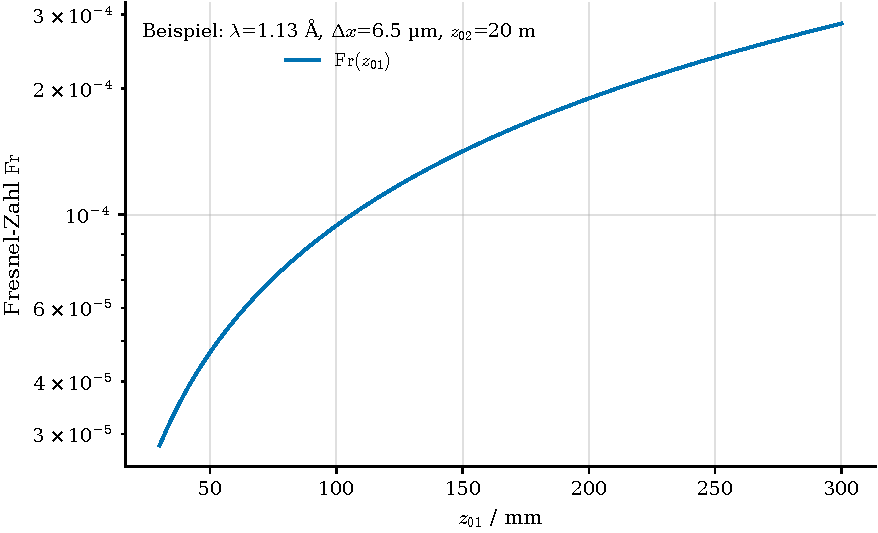
\includegraphics[width=0.8\textwidth]{figures/grundlagen/fresnelzahl}
  \caption[\lang{Fresnel-Zahl als Funktion des Abstands $\zOne$}{Fresnel number as a function of the distance $\zOne$}]{%
    \lang{Fresnel-Zahl $\Fr$ nach \cref{eq:grundlagen:fresnelzahl} als Funktion des
    Quelle--Objekt-Abstands $\zOne$ für Parameter in der Größenordnung des
    P05-Aufbaus ($\wl = \qty{1.13}{\angstrom}$ bzw.\ \qty{11}{\kilo\electronvolt},
    $\dx = \qty{6.5}{\micro\metre}$, $\zTwo = \qty{20}{\metre}$;
    vgl.\ \cite{dora2025autofocus}). Beispielabbildung im Stil
    \texttt{thesis.mplstyle}; durch eine echte Abbildung ersetzen.}%
    {Fresnel number $\Fr$ according to \cref{eq:grundlagen:fresnelzahl} as a
    function of the source--object distance $\zOne$ for parameters of the order
    of the P05 setup ($\wl = \qty{1.13}{\angstrom}$, i.e.\ \qty{11}{\kilo\electronvolt},
    $\dx = \qty{6.5}{\micro\metre}$, $\zTwo = \qty{20}{\metre}$;
    cf.\ \cite{dora2025autofocus}). Example figure in the
    \texttt{thesis.mplstyle} style; replace with a real figure.}}
  \label{fig:grundlagen:fresnelzahl}
\end{figure}

% ---------------------------------------------------------------------------
\begin{figure}[htbp]
  \centering
  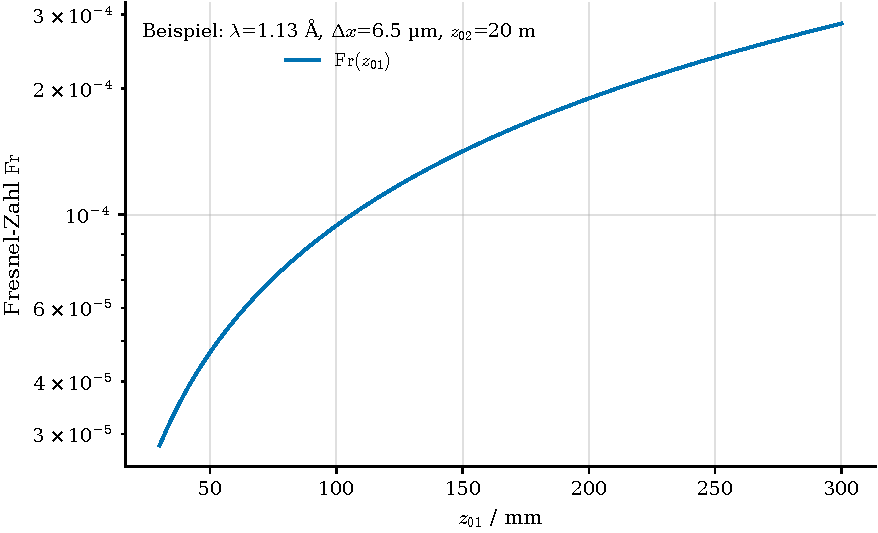
\includegraphics[width=0.8\textwidth]{figures/grundlagen/fresnelzahl}
  \caption[\lang{Fresnel-Zahl als Funktion des Abstands $\zOne$}{Fresnel number as a function of the distance $\zOne$}]{%
    \lang{Fresnel-Zahl $\Fr$ nach \cref{eq:grundlagen:fresnelzahl} als Funktion des
    Quelle--Objekt-Abstands $\zOne$ für Parameter in der Größenordnung des
    P05-Aufbaus ($\wl = \qty{1.13}{\angstrom}$ bzw.\ \qty{11}{\kilo\electronvolt},
    $\dx = \qty{6.5}{\micro\metre}$, $\zTwo = \qty{20}{\metre}$;
    vgl.\ \cite{dora2025autofocus}). Beispielabbildung im Stil
    \texttt{thesis.mplstyle}; durch eine echte Abbildung ersetzen.}%
    {Fresnel number $\Fr$ according to \cref{eq:grundlagen:fresnelzahl} as a
    function of the source--object distance $\zOne$ for parameters of the order
    of the P05 setup ($\wl = \qty{1.13}{\angstrom}$, i.e.\ \qty{11}{\kilo\electronvolt},
    $\dx = \qty{6.5}{\micro\metre}$, $\zTwo = \qty{20}{\metre}$;
    cf.\ \cite{dora2025autofocus}). Example figure in the
    \texttt{thesis.mplstyle} style; replace with a real figure.}}
  \label{fig:grundlagen:fresnelzahl}
\end{figure}

% ---------------------------------------------------------------------------
\begin{figure}[htbp]
  \centering
  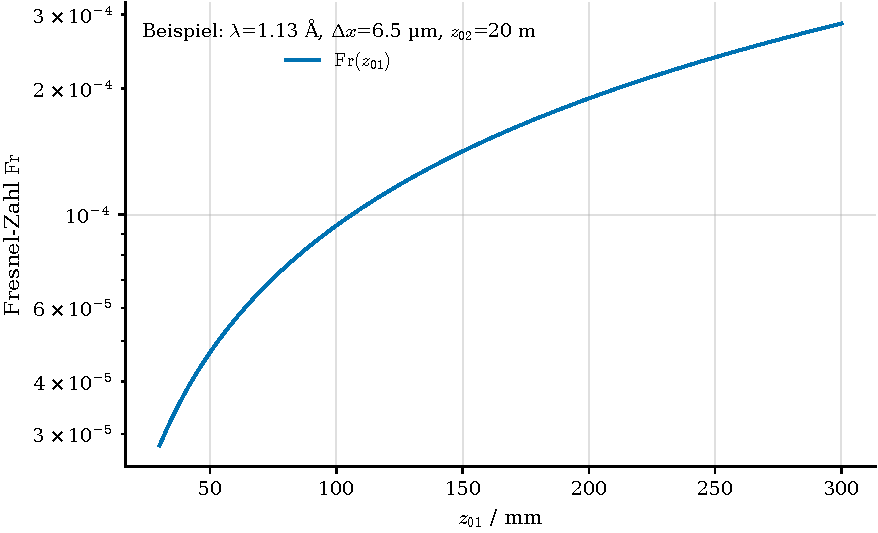
\includegraphics[width=0.8\textwidth]{figures/grundlagen/fresnelzahl}
  \caption[\lang{Fresnel-Zahl als Funktion des Abstands $\zOne$}{Fresnel number as a function of the distance $\zOne$}]{%
    \lang{Fresnel-Zahl $\Fr$ nach \cref{eq:grundlagen:fresnelzahl} als Funktion des
    Quelle--Objekt-Abstands $\zOne$ für Parameter in der Größenordnung des
    P05-Aufbaus ($\wl = \qty{1.13}{\angstrom}$ bzw.\ \qty{11}{\kilo\electronvolt},
    $\dx = \qty{6.5}{\micro\metre}$, $\zTwo = \qty{20}{\metre}$;
    vgl.\ \cite{dora2025autofocus}). Beispielabbildung im Stil
    \texttt{thesis.mplstyle}; durch eine echte Abbildung ersetzen.}%
    {Fresnel number $\Fr$ according to \cref{eq:grundlagen:fresnelzahl} as a
    function of the source--object distance $\zOne$ for parameters of the order
    of the P05 setup ($\wl = \qty{1.13}{\angstrom}$, i.e.\ \qty{11}{\kilo\electronvolt},
    $\dx = \qty{6.5}{\micro\metre}$, $\zTwo = \qty{20}{\metre}$;
    cf.\ \cite{dora2025autofocus}). Example figure in the
    \texttt{thesis.mplstyle} style; replace with a real figure.}}
  \label{fig:grundlagen:fresnelzahl}
\end{figure}

% ---------------------------------------------------------------------------
\begin{figure}[htbp]
  \centering
  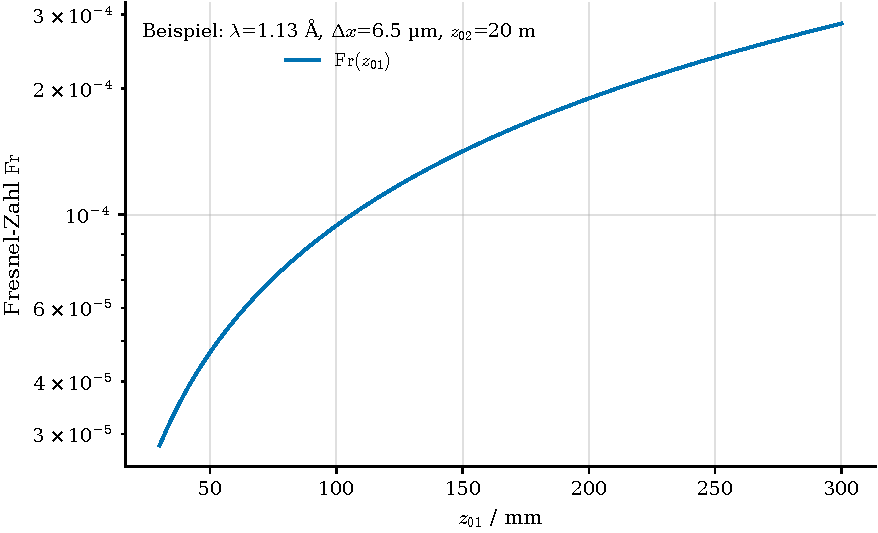
\includegraphics[width=0.8\textwidth]{figures/grundlagen/fresnelzahl}
  \caption[\lang{Fresnel-Zahl als Funktion des Abstands $\zOne$}{Fresnel number as a function of the distance $\zOne$}]{%
    \lang{Fresnel-Zahl $\Fr$ nach \cref{eq:grundlagen:fresnelzahl} als Funktion des
    Quelle--Objekt-Abstands $\zOne$ für Parameter in der Größenordnung des
    P05-Aufbaus ($\wl = \qty{1.13}{\angstrom}$ bzw.\ \qty{11}{\kilo\electronvolt},
    $\dx = \qty{6.5}{\micro\metre}$, $\zTwo = \qty{20}{\metre}$;
    vgl.\ \cite{dora2025autofocus}). Beispielabbildung im Stil
    \texttt{thesis.mplstyle}; durch eine echte Abbildung ersetzen.}%
    {Fresnel number $\Fr$ according to \cref{eq:grundlagen:fresnelzahl} as a
    function of the source--object distance $\zOne$ for parameters of the order
    of the P05 setup ($\wl = \qty{1.13}{\angstrom}$, i.e.\ \qty{11}{\kilo\electronvolt},
    $\dx = \qty{6.5}{\micro\metre}$, $\zTwo = \qty{20}{\metre}$;
    cf.\ \cite{dora2025autofocus}). Example figure in the
    \texttt{thesis.mplstyle} style; replace with a real figure.}}
  \label{fig:grundlagen:fresnelzahl}
\end{figure}
